
\documentclass{standalone}
\usepackage{tikz}
\usepackage{verbatim}
\begin{document}
\def\layersep{2.5cm}
    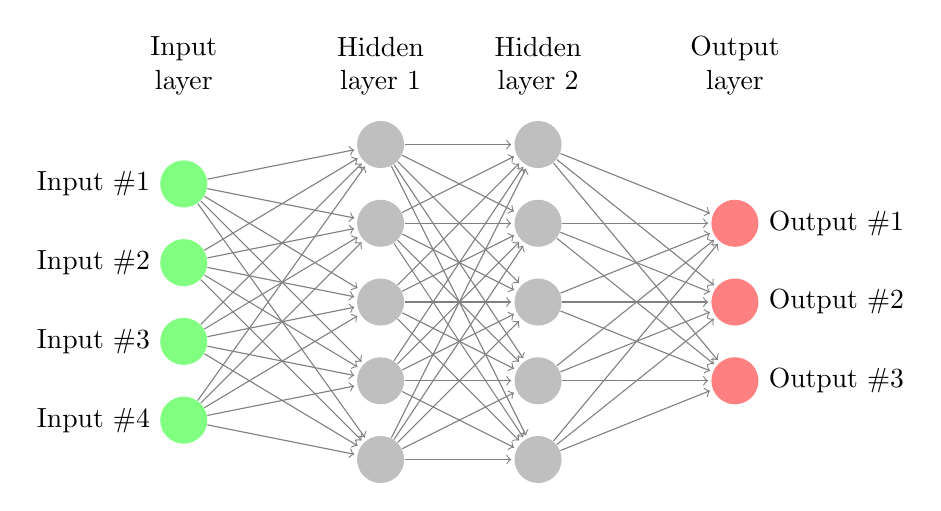
\begin{tikzpicture}[shorten >=1pt,->,draw=black!50, node distance=2.5cm]
        \tikzstyle{every pin edge}=[<-,shorten <=1pt]
        \tikzstyle{neuron}=[
            circle,fill=black!25,minimum size=17pt,inner sep=0pt
        ]
        \tikzstyle{input neuron}=[neuron, fill=green!50];
        \tikzstyle{output neuron}=[neuron, fill=red!50];
        \tikzstyle{hidden neuron}=[neuron, fill=gray!50];
        \tikzstyle{annot} = [text width=4em, text centered]

        % Draw the input layer nodes
        \foreach \id in {1,...,4}
        % This is the same as writing \foreach \name / \id in {1/1,2/2,3/3,4/4}
            \node[input neuron, label=left:{Input \#\id}]
                (I-\id) at (0,-\id) {};

        % Draw the hidden layers nodes
        \foreach \id in {1,...,5}
            \path[yshift=0.5cm]
                node[hidden neuron] (H1-\id) at (2.5cm,-\id cm) {};

        \foreach \id in {1,...,5}
            \path[yshift=0.5cm]
                node[hidden neuron] (H2-\id) at (4.5cm,-\id cm) {};

        % Draw the output layer nodes
        \foreach \id / \z in {1/2, 2/3, 3/4}
            \node[output neuron,label={right:Output \#\id}, right of=H2-\z]
                (O\id) {};

        % Connect every node in the input layer with every node in the first
        % hidden layer.
        \foreach \source in {1,...,4}
            \foreach \dest in {1,...,5}
                \path (I-\source) edge (H1-\dest);

        % Connect every node in the first hidden layer with every node in the
        % second hidden layer.
        \foreach \source in {1,...,5}
            \foreach \dest in {1,...,5}
                \path (H1-\source) edge (H2-\dest);

        % Connect every node in the hidden layer with the output layer
        \foreach \source in {1,...,5}
            \foreach \dest in {1,...,3}
                \path (H2-\source) edge (O\dest);

        % Annotate the layers
        \node[annot,above of=H1-1, node distance=1cm] (hl) {Hidden layer 1};
        \node[annot,above of=H2-1, node distance=1cm] (h2) {Hidden layer 2};
        \node[annot,left of=hl] {Input layer};
        \node[annot,right of=h2] {Output layer};
    \end{tikzpicture}% End of code
\end{document}